 \documentclass[12pt,english]{article}
\usepackage[utf8]{inputenc}
\markright{Pearse et al.\hfill Assessing the Effects Imputation on ED Values\hfill}
\usepackage{geometry}
\geometry{verbose,letterpaper,tmargin=2.54cm,bmargin=2.54cm,lmargin=2.54cm,rmargin=2.54cm}
%\geometry{verbose,letterpaper,tmargin=.1cm,bmargin=.1cm,lmargin=.1cm,rmargin=.1cm}
\usepackage{graphicx}
\DeclareGraphicsExtensions{.pdf,.png,.jpg}
\usepackage{amssymb,amsmath}
\usepackage{epstopdf}
\usepackage{tocbibind}
\usepackage[toc,page]{appendix}
\usepackage{supertabular}
\DeclareGraphicsRule{.tif}{png}{.png}{`convert #1 `dirname #1`/`basename #1 .tif`.png}
\usepackage{url}
\usepackage{subcaption}
\usepackage{caption}
\usepackage[super]{nth}
\usepackage{lineno} \linenumbers
\usepackage[doublespacing]{setspace}
\usepackage[parfill]{parskip}
\setlength{\parindent}{0pt}
\usepackage[citestyle=authoryear,bibstyle=authoryear,sorting=nyt,maxcitenames=2,maxbibnames=10,minbibnames=6,doi=false,url=false,isbn=false,firstinits=true,uniquename=false,uniquelist=false]{biblatex}
\bibliography{edge_sims}
\renewbibmacro*{name:andothers}{% Based on name:andothers from biblatex.def
  \ifboolexpr{
    test {\ifnumequal{\value{listcount}}{\value{liststop}}}
    and
    test \ifmorenames
  }
    {\ifnumgreater{\value{liststop}}{1}
       {\finalandcomma}
       {}%
     \andothersdelim\bibstring[]{andothers}}
    {}}
\renewcommand*{\finalnamedelim}{%
  \ifnumgreater{\value{liststop}}{2}{\finalandcomma}{}%
  \addspace\&\space}
\renewbibmacro{in:}{}
\AtEveryBibitem{%
  \clearfield{day}%
  \clearfield{month}%
  \clearfield{endday}%
  \clearfield{endmonth}%
}
\DeclareFieldFormat[article]{citetitle}{#1}
\DeclareFieldFormat[article]{title}{#1}
\DeclareFieldFormat[article]{pages}{#1}
\DeclareNameAlias{sortname}{last-first}

\usepackage{changes}
\setdeletedmarkup{\textcolor{red}{\sout{#1}}}

\begin{document}
\setlength{\parindent}{0pt}
\section*{Title page}

\textbf{Article title}: Assessing the Effects Imputation on ED Values

\textbf{Running head}: Assessing the Effects Imputation on ED Values

\textbf{Authors:} K.\ Bodie Weedop$^{1}$, William D.\ Pearse$^{1}$\

$^1$ Department of Biology \& Ecology Center, Utah State University,
5305 Old Main Hill, Logan UT, 84322

$^*$To whom correspondence should be addressed:
\url{will.pearse@usu.edu}

\textbf{Word-count}: 5680 (abstract, main text, acknowledgements, and
  references)

\clearpage
\section*{Abstract}


\textbf{Keywords}: 

\clearpage
\section*{Introduction}
Evidence from the fossil record and present-day studies argue we are in the
midst of, or entering, a sixth mass extinction
\autocite{Barnosky2011, Ceballos2015}, such that more species than ever are
declining and/or in danger of extinction across a range of environments
\autocite{Wake2008,Thomas2004}. Habitat destruction
\autocite{Brooks2002}, invasive species \autocite{Molnar2008}, climate change
\autocite{Pounds2006}, and disease \autocite{Lips2006} are some of the leading
causes of species declines globally. Conservation biologists seek to reverse
these declines and their detrimental effects on species populations, but in
reality they have limited resources with which to do so. This challenge, termed
the ``Noah's Ark problem'' \autocite{Weitzman1998}. The concept of conservation
prioritization, or conservation triage, has provided an efficient method of
allocating resources to confront this issue \autocite{Bottrill2008}. 

Conservation triage requires decision making supported by some metric
quantifying the importance and degree of endangerment urgency for a set of
species. By using such a metric, researchers are able to remove themselves and
any potential bias from the allocation of time and resources for conservation.
One of these triage strategies which have been introduced and used most widely
is the EDGE metric\autocite[Evolutionary Distinction and Globally
Endangered;][]{Isaac2007}. This method prioritizes species according to two
metrics: Evolutionary Distinctiveness (ED) and Global Endangerment (GE). ED
measures relative contributions to phylogenetic diversity made by each species
within a particular clade\autocite{Isaac2007}. Such contributions are assessed
by quantifying the amount of branch length which is unique to each species
within the overall phylogeny. GE values are assessed by assigning numerical
values to each of the World Conservation Union (IUCN) Red List Categories. These
numerical values are assigned through transforming the IUCN Red List categories
into probabilities of extinction \autocite{Mooers2008}. As species become
increasingly threatened and are placed into more concerning categories
(\emph{e.g.}, from Vulnerable to Endangered), the GE numerical value increases.
Increases in either ED or GE place a particular species at a higher priority for
conservation effort.

EDGE has been applied in order to prioritize a number of species groups in the
recent past since its' initial deployment. Some of these applications include
applying EDGE to mammals \autocite{Isaac2007}, amphibians \autocite{Isaac2012},
and more recently for bird species \autocite{Jetz2014} and corals
\autocite{Curnick2015}. Alongside EDGE there have been a number of similar
metrics which have been developed and some discussion of which should be used
over others \autocite{Steel2007, Pearse2015}. Apart from discussion of preferred
metrics, there is also discussion of whether likelihood of success in
conservation \autocite{arg}, relative cost of certain interventions
\autocite{arg}, and complementarity of interventions \autocite{arg} should also
be accounted for when designing metrics used going into the future. EDGE is
limited in this regard; it does not include these nuanced factors from which it
may benefit. However, EDGE has formed the basis for a successful program which
addresses conservation in a quantitative manner. EDGE has provided actionable
insights for conservation effort to be focused upon widely unknown species. It
has established that phylogenetic conservation prioritization metrics can be
used by conservation biologists and policy makers alike. Nonetheless, each
application of EDGE has dealt with the uncertainty presented by missing species
data.

% Some of the text in this paragraph will now be pulled into the one
% above. You'll also find that you'll now be able to talk in a little
% bit more detail about *how* imputation takes place, citing the Kuhn
% polytomy paper and the Jetz paper, I suppose. Does that make sense?
In the event of missing DNA or trait data, species are often difficult or not
able to be placed onto a phylogeny. Even in the face of such uncertainty and
missing data, it is understandable that conservation biologists want to make
prioritizations. However, if we are using a quantitative method for prioritizing
species, we should remain consistent even when uncertainty arises. To our
knowledge, a proper and efficient method for prioritizing species where there is
missing data is still untested. This issue pertains mainly to the calculation of
ED than GE. The IUCN has collected data on most major clades, and has a strategy
for assigning Red Listing values these species which we know little information
and are considered Data Deficient (DD). IUCN and other conservation
organizations support focus on DD species just the same as Critically Endangered
and Endangered species to ensure consistency \autocite{Rodrigues2006}. However,
to our knowledge, there has been no systematic investigation of the efficacy of
such imputation, both in terms of the accuracy with which imputed ED values are
estimated, and the effect on other known species' scores. Indeed, it is unclear
whether any significant information on ED is gained by imputing species which
cannot be placed on the phylogeny. It is also not well understood how simply
removing missing species, compared to performing imputation, would effect ED
values. It may be that simply excluding missing species may be less intrusive
than imputation. In searching for a solution for missing species, we may be
negatively affecting correct ED values and disrupting EDGE rankings in the
process. As the desire to use ED and phylogenies for conservation triage grows,
the importance of such tests and a consensus on how to resolve cases of
phylogenetic uncertainty becomes more urgent.

Our aim is to test of how missing species data affects EDGE rankings and assess
whether imputing species is a defensible method for dealing with species not
easily placed on the phylogeny. The uncertainty of missing species data was
replicated by removing species from simulated trees in two ways: at random and
in a phylogenetically biased manner. By doing so, we hope to provide a model of
how EDGE values are affected when species difficult to place on a phylogeny are
excluded. Also, we assess the extent to which EDGE rankings based upon imputed
phylogenies can be used within applied conservation biology. To do this, we
replicate the imputation approach by randomly removing, replicating, and
replacing one particular clade all under the same model of evolution. In doing
so, we hope to understand the effect that imputation has on ED values and offer
some discussion of whether it is a viable solution for dealing with missing data
species. We found that ED values throughout the tree are affected by excluding
missing species from the phylogeny \ref{randomVsClustered}. Also, we found no
correlation between imputed and true ED values for a species within an imputed
clade (\ref{imputationTrend}; Table 2). 

\section*{Methods}
Here we use a simulation approach to test the effect of removing and imputing
species on a phylogeny on subsequent ED (Evolutionary Distinctiveness) scores of
species. Since empirical studies do not (to our knowledge) impute GE (Global
Endangerment) scores for species, and our focus here is on the importance of
phylogenetic structure, we focus on the impact of imputing ED values. EDGE is
the product of both ED and GE, any true GE values assigned will remain biased by
any inaccuracy in ED values due to imputation.

All simulations and analyses were performed using R \autocite[version
3.4.0;][]{R2017}}. For each combination of parameter values in a simulation, we
performed 100 replicate simulations. Original and manipulated trees were
simulated under a pure-birth Yule model using the \texttt{sim.bdtree} function
\texttt{geiger} R package \autocite{Harmon2007}. This particular model was
chosen because it is the simplest model possible; each branch is associated with
only one value: birth rate. If excluding or imputing missing species shows to be
ineffective under this particular model of evolution, it will most likely not be
effective in more complex biological simulations. In order to calculate ED
values, the function \texttt{ed.calc} within the R package \texttt{caper} was
used to calculate ED values for each tree \autocite{Orme2013}.

% I moved the part where I am talking about imputing the clade under the
% same model of evolution to the subsection where it should be addressed more
% specifically
% - Bodie

\subsection*{Assessing the impact of missing species on EDGE-listing}
Our first set of simulations assesses the impact of random loss and
phylogenetically-biased loss of species on ED scores. We test both manners of
species loss in order to simulate both random selectivity and phylogenetic
selectivity in missing species data. Missing species at random was simulated by
selecting species at random without replacing, and removing those species from
the tree. This randomization had no regard for phylogenetic structure. Missing
species related by some character trait was tested by simulating character trait
values for each tip. These simulations were all performed under a constant rate
Brownian-motion model (\sigma$^2$=0.5, starting root value = 1). Tips were
dropped if their character trait values place them into the upper quantile which
had been selected to be dropped. More specifically, if the fraction to be
dropped was 10\%, species within the 90th quantile of character trait values
were dropped. Both sets of simulations were carried out using phylogenies of
different sizes (number of taxa: 64, 128, 256, ..., 2048, 4096), removing
constant fractions of tips from the tree (0\%, 1\%, 2\%, ..., 19\%, 20\%).

We assessed the impact that removing missing species has upon ED values using
the correlation of all ED values for the tips remaining within both trees. To
evaluate the effect that imputation has upon ED values, we calculated ED for all
tips in both the original and manipulated trees while excluding the focal clade
where imputation has occurred. These ED values were compared using a
correlation. Additionally, we did the same calculations and comparison using
only the original focal clade and its' simulated replacement. If missing species
have no effect upon ED values, we expect a high, positive coefficient of
correlation between the original tree and its' manipulated counterpart.
\added{state why this model is a useful one---re-state the propoerty it has,
  linking it back to why this is a useful set of simulations to be doing}. 

% Do you need to repeat this with different sigma values?
% Hmmm, what?? -Bodie
% Also, this parameter is sigma squared, right? Yes, thanks -Bodie
% Re-write the next two sentences - be specific the first time you
% state it.

\subsection*{Assessing the impact of phylogenetic imputations}
We tested the impact of imputing missing species onto a clade of a particular
size (sizes 3, 4, 5, ..., 30, 31, 32) which originated from a tree of a
particular size (number of taxa = 64, 128, 256, 512, 1024). To simulate the
effect that phylogenetic imputation has upon EDGE rankings, we randomly selected
one clade to be removed from the original tree, simulated a new separate tree of
the same size under the pure-birth model used before, and placed the newly
simulated clade back where the original clade was removed. Thus we have imputed
each clade under the same model used to generate it. In an empirical study, this
would be done by assigning all the species of the resolved clade the mean ED
value obtained from all possible or numerous resolutions of the clade.
Therefore, our method is being generous because the numerous resolutions of that
clade would be produced under a model which would have to be estimated. By doing
this, we replicated the process of imputation of a clade which has been
resolved. 

To assess whether clades, once imputed, had similar ED scores, we
correlated the imputed ED scores against true ED scores. We also looked at ranks
to understand the amount of error introduced when imputing species. We
statistically modelled these as a function of the number of total species and
number of species within an imputed clade, hypothesizing that each would matter
because the erroneous ranking of imputed species would range across the total
amount of species depending on the amount of species imputed.

\section*{Results}
Under both random and phylogenetically-patterned loss, ED values of remaining
species are affected by the total number of species removed (Table 1;
\ref{randomVsClustered}. In either case, a similar effect on the correlation
between remaining ED values before and after species are removed is seen.  

\begin{figure}[!ht]
  \center
  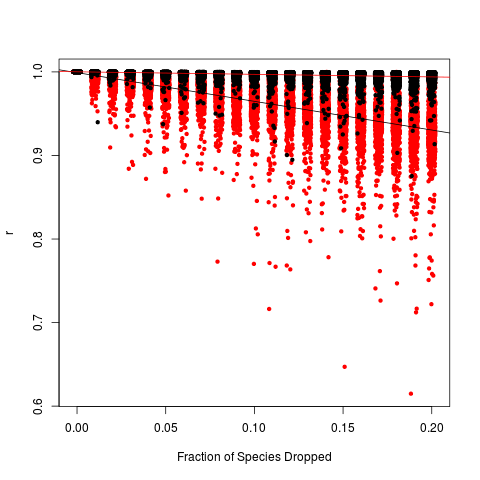
\includegraphics[width=.5\textwidth]{randomVsCluster.png}
  \caption{\textbf{R-values plotted against the fraction of species dropped at
  random versus clustered manner.} The color of data points denote whether
  species were dropped at random (orange; n = 100) or in clustered manner
  (grey; n = 100). The regression lines are demonstrating the relationship when
  species are dropped at random (red) and in a clustered manner (clustered). The
  correlations represent a comparison of the ED values (before and after
  species are dropped) of species which remain on the on the phylogeny after
  other species are dropped. 
  }
  \label{randomVsClustered}
\end{figure}

\begin{table}[ht]
  \centering
  \begin{tabular}{rrrrr}
    \hline
      & Estimate & Std. Error & t value & Pr($>$$|$t$|$) \\
      \hline
      (Intercept) & 1.0315 & 0.0013 & 821.39 & $<$0.0001 \\
      Fraction of Species Dropped & -0.4696 & 0.0020 & -233.16 & $<$0.0001 \\
      Random Treatment & 0.0630 & 0.0018 & 35.47 & $<$0.0001 \\
      Number of Species Overall & 0.0000 & 0.0000 & 7.89 & $<$0.0001 \\
      Fraction of Species Dropped:Random Treatment & -0.2774 & 0.0028 & -97.45 & $<$0.0001 \\
      Random Treatment:Number of Species Overall & 0.0000 & 0.0000 & -4.38 & $<$0.0001 \\
      \hline
    \hline
  \end{tabular}
\caption*{\textbf{Table 1: ANCOVA model summary describing the effect of
dropping species on remaining species ED Values.} The fraction of species
dropped significantly affects the the remaining ED values. Dropping the
fraction both at random and in clustered manner both have negative effects on
the remaining ED values ($F_{139696, 5}$ = 40350, $R^{2}$ = 0.5908,
p$<$0.0001).}
\end{table}

We find no support for a correlation between the imputed and true ED values for
a species within an imputed clade (\ref{imputationTrend}, table 2). We
do find evidence that, when imputing larger clades, the variation in the
correlation is lesser (quantile regression), but this could be due to XXX. We
% I need to do the quantile regression... -Bodie 
found that measures of the true phylogeny such as phylogentic diversity (PD),
lambda, Colless' Index, skew, and kurtosis do not provide any indication that
imputation would negatively affect ED values (Appendix A). Just as imputed ED
values did not reflect true ED values, the rankings of species within the focal
clade were altered significantly under imputation (Fig. \ref{rankingError};
Table 3). Our model suggests that with increases in the size of the imputed
clade and overall number of species, species within the clade are ranked farther
from their true ranking (Table 3). Also, this same effect is seen in the error
rate within top ranking species (Appendix B).

\begin{figure}[!ht]
  \center
  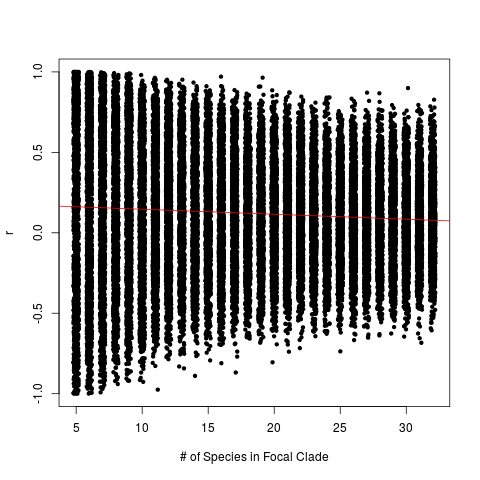
\includegraphics[width=.5\textwidth]{edModel.png}
  \caption{\textbf{R-values plotted against the number of species at focal
  clade.} Each data point denotes a correlative comparison between ED values
  within the focal clades where imputation has occurred. The regression line
  (red) and trend even closer to zero demonstrates the decrease in informative
  value of the imputed ED values. This is reinforced by the visual narrowing of
  r-values around zero.}
  \label{imputationTrend}
\end{figure}

\begin{table}[ht] 
\centering
\begin{tabular}{rrrrr}
  \hline
  & Estimate & Std. Error & t value & Pr($>$$|$t$|$) \\
   \hline
 (Intercept) & 0.1852 & 0.0533 & 3.47 & 0.0005 \\
   Size of Focal Clade & -0.0034 & 0.0002 & -16.56 & 0.0000 \\
   Size of Phylogeny & -0.0001 & 0.0001 & -0.41 & 0.6855 \\
   PD & 0.0001 & 0.0001 & 0.37 & 0.7108 \\
   Lambda & -0.0012 & 0.0524 & -0.02 & 0.9812 \\
   Colless' Index & 0.0016 & 0.0022 & 0.72 & 0.4687 \\
   Skew & 0.0043 & 0.0088 & 0.48 & 0.6288 \\
   Kurtosis & -0.0005 & 0.0009 & -0.63 & 0.5269 \\
   \hline
   \hline
\end{tabular}
\caption*{\textbf{Table 2: Effect of Clade Size on Imputed ED Values.} The
intercept describes that the correlation between the true and imputed values
begins quite low. As the clade size increases, this correlation only tends
toward zero. The total number of species in the full phylogeny along with
measures of the true phylogenetic diversity, lambda, Colless' Index, skew, and
kurtosis show no significant effect. ($F_{47992, 7}$ = 39.57, $R^{2}$ = 0.006,
p$<$0.0001).}
\end{table}

\begin{figure}[!ht]
  \center
  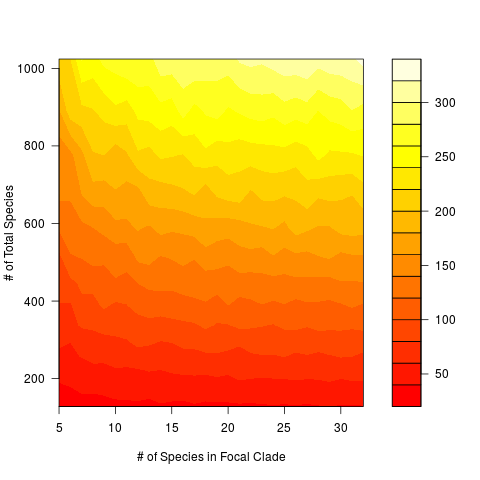
\includegraphics[width=.5\textwidth]{rankingError.png}
  \caption{\textbf{Mean ranking error of species within the focal clade.} The 
  gradient on the right demonstrates average number of posistions within the 
  full ranking that focal clade species shifted from their true rank.
  While controlling for the size of the full phylogeny and focal clade, species 
  within the focal clade were, on average, ranked far from the true rank. }
  \label{rankingError}
\end{figure}

\begin{table}[ht]
  \centering
  \begin{tabular}{rrrrr}
    \hline
   & Estimate & Std. Error & t value & Pr($>$$|$t$|$) \\
    \hline
  (Intercept) & -1.6344 & 0.0332 & -49.29 & 0.0001 \\
    Size of Focal Clade & 0.0900 & 0.0010 & 91.22 & 0.0001 \\
    Size of Phylogeny & 0.5179 & 0.0013 & 383.99 & 0.0001 \\
     \hline
     \hline
  \end{tabular}
  \caption*{\textbf{Table 3: Effect of Clade Size and Total Species on Ranking
  Error.} Model demonstrating the relationship between focal clade species
  ranking error and the size of imputed clade and overall phylogeny. Square-root
  transformations have been applied to both ranking error and size of phylogeny.
  Significant increases ranking error are seen when increasing sizes of both the
  imputed clade and phylogeny ($F_{47997, 2}$ = 77890, $R^{2}$ = 0.7644,
  p$<$0.0001).}
  \end{table}

\clearpage
\section*{Discussion}
Phylogenetic conservation prioritization is an emerging tool providing a much
needed, objective measure for conservation decision-making and policy. However,
phylogenetic uncertainty is a major obstacle for EDGE and similar metrics
\autocite{Collen2015}. Uncertainty in phylogenies could mean that species in
desperate need of conservation effort are overlooked. In order to address such
uncertainty, we aim to determine how removing missing species from a phylogeny
affects ED values for the remaining species and demonstrate how imputation
affects ED values of species where imputation is performed. Our results
demonstrate that missing a proportion of overall species both at random and in a
phylogenetic-biased manner have different yet significant affects on remaining
ED values throughout the tree and imputation does not recover the ED value or ED
rank of an imputed species.

Our results are derived solely from simulations under a simple model of
diversification---the Yule model. We do acknowledge that, in the real world,
lineages evolve in more complex ways than are captured by such a simple model.
While we do not have empirical data, imputing species under this model should be
much easier given the simplicity. We have not been given any implication through
this investigation that a more complex model would produce any different result.
Therefore, we suggest that our results generalize from the simplest case to more
complicated cases which might be seen in empirical data. However, our results
demonstrate that even under a simple model imputing species lead to a
misrepresentation of true ED values. 

Nomrally, imputation is averaged across all numerous trees to get the closest
estimate of true ED values. However, imputed trees still deviate from the true
trees and therefore the average would also be far from the true average.
% Describe in a single sentence how imputation takes place across the
% posterior distribution of trees. Point out that our results show
% there is uncertainty in that distribution of trees, which is our
% focus.

\subsection*{Uncertainty in imputed species}
Missing species and poor phylogenetic resolution have been identified as causes
of uncertainty when calculating ED \autocite{Isaac2007}. Prior to our
investigation, we could not find any assessment of how missing species might
affect ED values of species which are not missing. In previous research,
incomplete phylogenies were shown to produce nearly the same result as the
later, more complete trees \autocite{Curnick2015}. While demonstating EDGE
scores derived in the face of phylogenetic uncertainty still perform quite well
in setting accurate priorities, they did not explicitly test the effect which
missing species, nor imputing missing species, has on ED values. 

% Does it? The curves are very similar to me. See my comment below: if
% you give something quantitative, it's going to be easier for the
% reader to do something with this. 

We realize that we have provided just two ways in which species could be missing
from a phylogeny and there are more that could occur. Missing species could be
biased by some phylogenetic pattern other than Brownian motion evolution.
Nevertheless, our investigation shows that missing species cause ED values of
species remaining in the phylogeny to deviate from the true value.
% I would frame this in exactly the same way as you should frame the
% Yule model thing. Say, yes, we realise this is a simple model, but
% it shows an effect, and so this is something to think about. I would
% speculate about the kind of model that would be interesting to look
% at further: perhaps one where species radiate in situ and stay in
% place. Thus you could be missing an entire clade and it would be in
% the same place. Maybe find some literature about how species tend to
% be missing from conservation prioritisation or phylogenies and then
% cite that. Just a few sentence of waffle, informed by the
% literature.

% I'll need to find and read some this literature... -Bodie 

In the past, we have included missing species into the EDGE framework using
different methods. Collen et al. assigned the mean ED score of presumed
congeneric species to the missing species \citeyear{Collen2011}. More
frequently, missing species and poorly resolved clades have been dealt with by
imputing the missing species and assigning all the species of the resolved clade
the mean ED value obtained from all possible or numerous resolutions of the
clade \autocite{Isaac2007; Isaac2012}. This method has been adapted by others
and applied where there were large percentages (~30\% or 3,330 species) missing
\autocite{Jetz2014}. 

While imputation does include missing species, research has
shown imputed phylogenetic data leads to biases in some ensuing analyses
\autocite{Rabosky2014}.
% You're being a bit vague again. Rabosky has some quite specific
% take-homes: report them. 

When considering the analysis of ED, our results show that imputation does not
recover true ED values nor ED rank of missing species \ref{imputationTrend;
rankingError}. As the size of the imputed clade increases, ED values of imputed
species do not correlate with their true values (Table 2). Even though we are
including missing species into calculating ED, we are not obtaining accurate
information about those species. While being uninformative, these ED values
would also lead to mispriortizing species based on our results. In the event
that a clade of 25 species in a phylogeny of 850 species, our results show those
imputed species would be, on average, 250 ranks from their true rank (Fig.
\ref{imputationTrend}; Table 3).
% Be specific and quote some quantitative information.
Analyzing the performance of imputation of a clade less than five
species was not performed due to limitations of statistical validity
\autocite{Crawley2012}.
% this is also vague, and makes it all sound a bit fishy. You can turn
% this into a point of strength, something like:
% * We do not report correlations when the clades were smaller than 5,
%   because we can't report a correlation reliably with so little data
% * But, it would be surprising if our trend suddenly changed such
%   that, when imputing only one species, it did better.
% * Invoke Arne's 'the clade should have an average ED' argument to
%   support this. In smaller clades (i.e., two species, and you don't
%   know where that species goes) then you should just be sampling from
%   the prior. That prior is exponential, and so there's absolutely no
%   reason to suppose it will do any better than what we have
%   already. This is a more complicated argument, so have a bash at it
%   and then we can talk.

Even so, our results provide no indication
that the effects of imputation seen in our results would improve when
applied at smaller clades.

\subsection*{Guidelines for the use of imputation}
We suggest there is a straightforward synthesis of these results that should be
useful in applied conservation biology. Both random and
phylogenetically-patterned loss of species affect ED values throughout the tree.
However, we found that ED values of non-missing species remain relatively
constant under imputation. Therefore, imputation could be used to avoid missing
species biasing ED values of non-missing species. We have shown that imputing
missing species would not provide accurate ED values for missing species.
However, it would provide a method of avoiding the loss of species affecting ED
values throughout the remainder of the tree. Basing conservation priorities upon
the ED values of imputed species would lead to inaccurate prioritization.
Nevertheless, imputation may be useful to stop missing species from biasing
species easily placed on the phylogeny.
% Make sure you reference the *result* that you have found - that the
% correlation of the non-imputed species is high. You could even
% explicitly compare it with the correlation when there's no
% imputation: if the correlation is better, good news! It's given us
% something. If it's not... well, we can worry about that if you find
% it :D

Given these results, we now present guidelines for how missing species should be
dealt with and when imputation might be appropriate when calculating EDGE. In
the event of missing species, researchers should be investigating the amount of
species that are missing and consider whether imputation is necessary. For some
context, in our analysis we found that if 30\% of species are missing at random
or in a phylogenetic-biased manner from the phylogeny, respectively, ~80\% and
~89\%. Therefore if species are missing, we should verify that the amount of
missing species does not exceed a percentage which we have found to provide poor
ED values for remaining species. While below an acceptable percentage of missing
species, EDGE should be carried out without attempting to impute the missing
species.
% This could be a very good idea; are you saying to see if the
% fraction you're missing is greater than the error that would be
% added in? Check what I'm saying about the r2, but it sounds like you
% could have found a very nice rule of thumb. I would even consider
% using the phrase "rule of thumb", as it will drive home to the
% reader that you're giving a guide to thought.
However, if a larger proportion of species are missing, imputation may
be used but with some caution. ED values for species easily placed on
the phylogeny are relatively unaffected and can be trusted when
setting conservation priorities. Nevertheless, ED values and ranks of
species which have been imputed should either be ignored or used
cautiously within EDGE.
% Bring in something quantitative here as well - reference the average
% error in ranking, and use that to give another 'rule of thumb' as to
% how variable the ranking could be for a species with no data. Does
% that make sense?
By following these guidelines we avoid biasing species which are
easily placed on the phylogeny even in the event that imputation is
used.

\section*{Acknowledgments}

\clearpage
\printbibliography

\clearpage
\appendix
\section*{A. Effect of Measures of the True, Full Phylogenies}

\begin{figure}[!ht]
  \center
  
\includegraphics[width=.5\textwidth]{trueColless.png}
  \caption{\textbf{Effect of the True Colless Index of FullPhylogeny.}}
\end{figure}

\begin{figure}[!ht]
  \center
  
\includegraphics[width=.5\textwidth]{trueLambda.png}
  \caption{\textbf{Effect of the True Lambda of Full Phylogeny.}}
\end{figure}

\begin{figure}[!ht]
  \center
  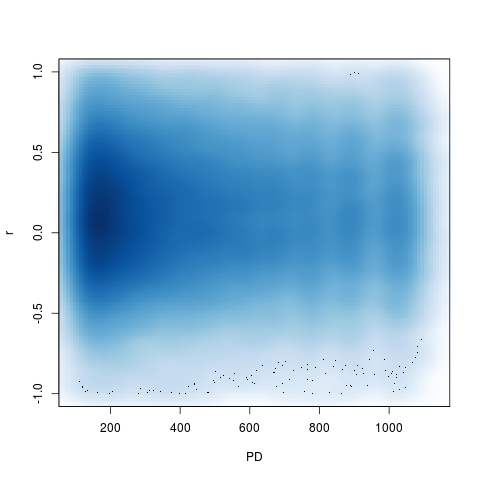
\includegraphics[width=.5\textwidth]{PD.png}
  \caption{\textbf{Effect of True PD of Full Phylogeny.}}
\end{figure}

\begin{figure}[!ht]
  \center
  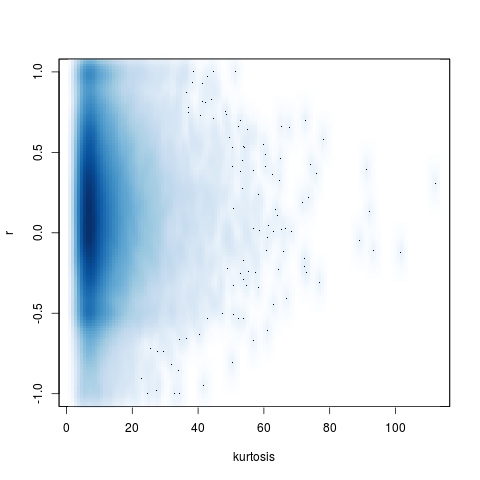
\includegraphics[width=.5\textwidth]{originalKurtosis.png}
  \caption{\textbf{Effect of the True Kurtosis of Full Phylogeny.}}
\end{figure}

\begin{figure}[!ht]
  \center
  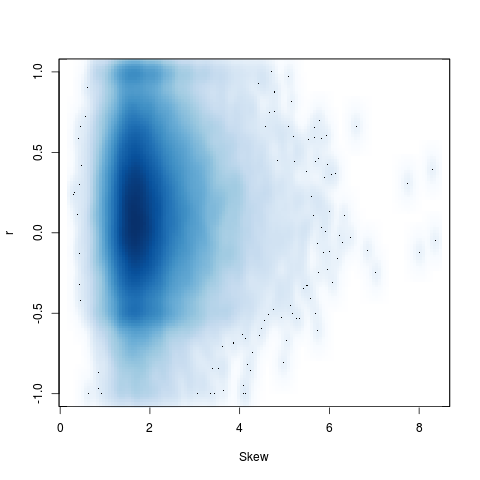
\includegraphics[width=.5\textwidth]{originalSkew.png}
  \caption{\textbf{Effect of the True Skew of Full Phylogeny.}}
\end{figure}

\clearpage
\clearpage
\section*{B. Error Rate in Top Rankings}

\begin{figure}[!ht]
  \center
  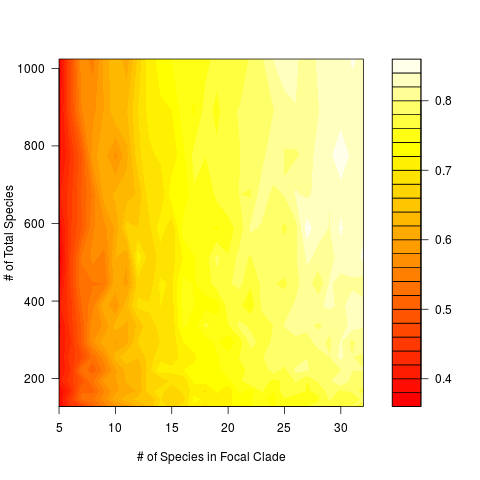
\includegraphics[width=.5\textwidth]{errorRate50.png}
  \caption{\textbf{Mean error rate in the ranking of top 50 species.}}
\end{figure}

\begin{figure}[!ht]
  \center
  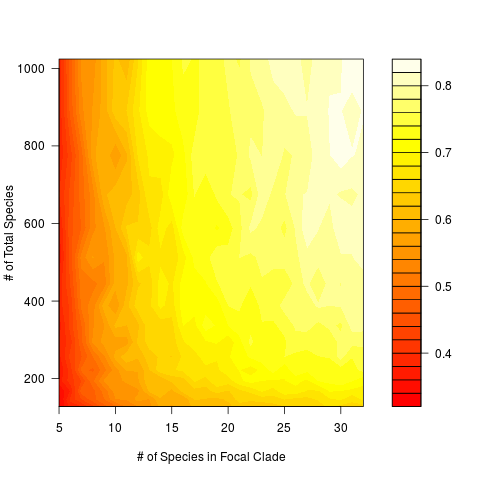
\includegraphics[width=.5\textwidth]{errorRate100.png}
  \caption{\textbf{Mean error rate in the ranking of top 100 species.} }
\end{figure}

\begin{figure}[!ht]
  \center
  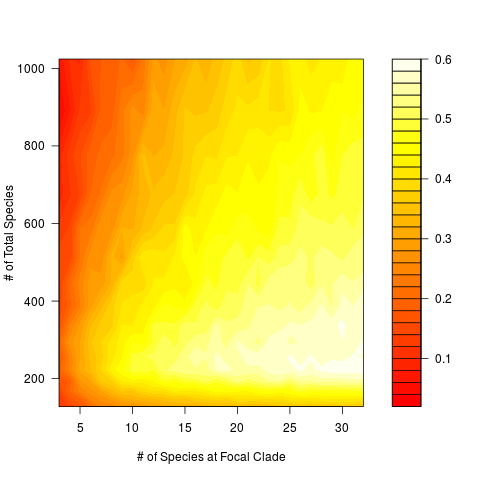
\includegraphics[width=.5\textwidth]{errorRate200.png}
  \caption{\textbf{Mean error rate in the ranking of top 200 species.} }
\end{figure}

\begin{figure}[!ht]
  \center
  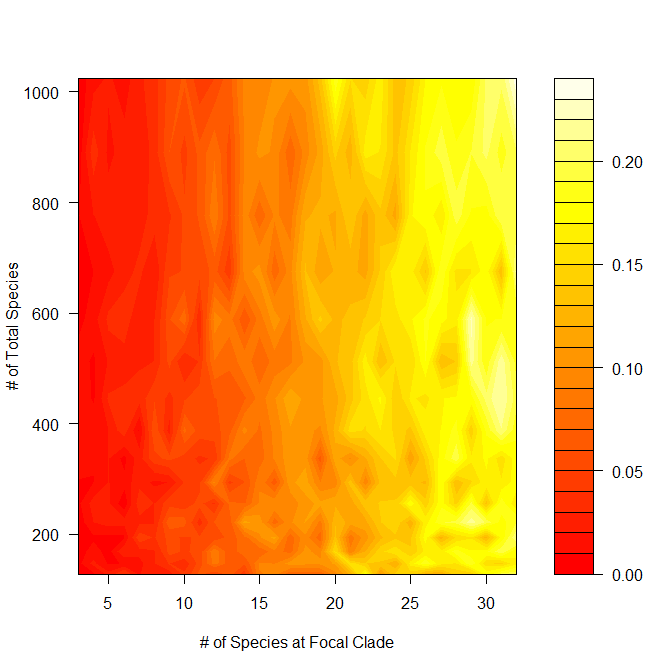
\includegraphics[width=.5\textwidth]{errorRate5pct.png}
  \caption{\textbf{Mean error rate in the ranking of top 5\% of species.} }
\end{figure}

\begin{figure}[!ht]
  \center
  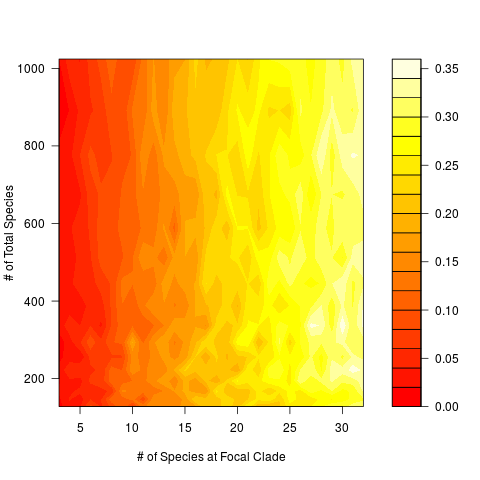
\includegraphics[width=.5\textwidth]{errorRate10pct.png}
  \caption{\textbf{Mean error rate in the ranking of top 10\% of species.} }
\end{figure}

\begin{figure}[!ht]
  \center
  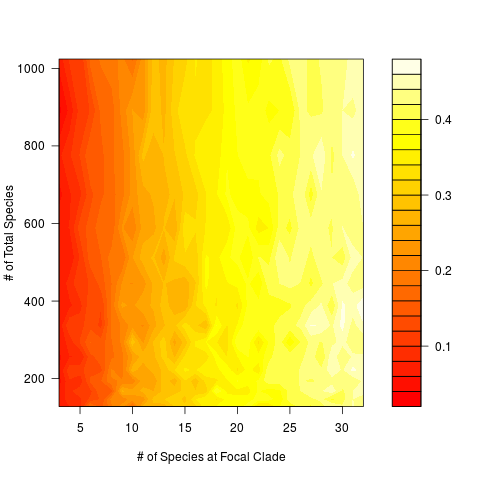
\includegraphics[width=.5\textwidth]{errorRate20pct.png}
  \caption{\textbf{Mean error rate in the ranking of top 20\% of species.}}
\end{figure}

\end{document}
%%% Local Variables:
%%% mode: latex
%%% TeX-master: t
%%% End: